\section{Process perspective} \label{pp}
%% Short introduction to this section. 
\subsection{Stages and tools in CI/CD} % micje
%% Include screenshots and/or UML diagram.
%% A somewhat detailed, but complete description of our Github Action flow for CI/CD. This also includes a description of our Github rules, and how releases were made.


\subsection{Monitoring} %% phbl
An important part of DevOps relates to operations, and ensuring that existing code is running as intended. Through monitoring, we are able to continuously check if our were active and processed incoming requests. For our setup, we have made use of Grafana as our visualisation tool, scraping information about our mini-twit application using the open-source web application scraper tool Prometheus. Prometheus scrapes information from the "/metrics" endpoint, created using the go package \texttt{ginprom}, and provides a multitude of information on the go application behind mini-twit represented using time series data. Prometheus maintains it own storage locally, and to ensure that replacing the mini-twit virtual machine does not lose its time series information, we created a dedicated volume in digital ocean to store this data, alongside the configuration files for Prometheus. 

%% Include screenshots
\subsection{Logging} %% phbl
While monitoring provides an overview of a system through metrics and health checks, we need to use logging to get more detailed information about events that have transpired, their timestamps and other relevant information. Our logging setup has been based around Grafana as a visualisation tool, Grafana Loki as a log aggregation tool, and Grafana Alloy as the logging tool. Our logging efforts were divided amongst our docker containers, reading their logs. In extension to this, we implemented logs for our mini-twit application using the standard logging library in Golang \texttt{slog}. Here we focused on implementing log events for all of our event handlers, since their process information was deemed most important. 

\begin{figure} [H]
    \centering
    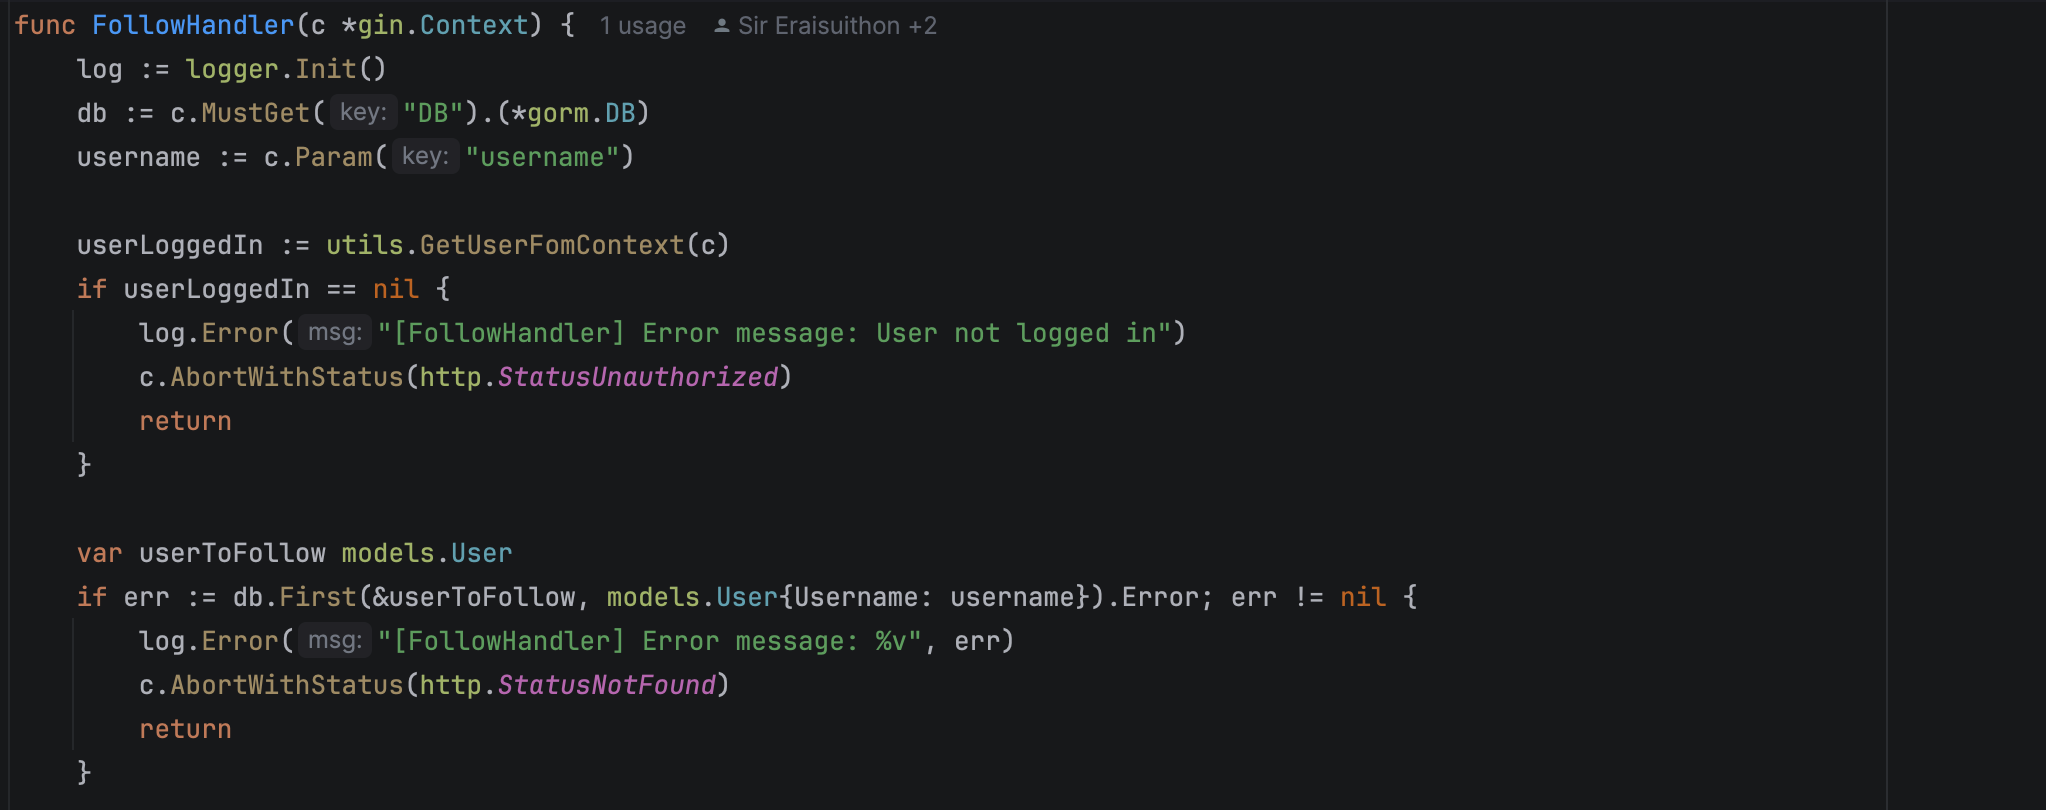
\includegraphics[width=1\linewidth]{pictures/StdLog.png}
    \caption{Example of logging with FollowHandler showcasing how errors are propagated as a log.}
    \label{fig:enter-label}
\end{figure}


%% Include screenshots
%% Description of Grafana logging dashboard... loki, alloy. 
\subsection{Security assessment} %% micje
%% A revision of the security assessment we did in an earlier exercise, how we took steps to improve as well as the risk matrix. 
To identify possible attack surfaces, we made a full port-scan of our server which came up with the following open ports;
\begin{description}
    \item[22] SSH
    \item[80, 443] web-app through traefik
    \item[3000] grafana
    \item[3100] loki
    \item[12345] alloy
    \item[9090] prometheus
\end{description}
We reasoned that the following were already secure; SSH, web-app, grafana and prometheus. That left Loki and All
\subsection{Scaling strategy} %% alpl
%% The use of swarm as a way to scale, rolling updates, etc.

\subsection{Use of Artificial Intelligence} %% phbl
In our project, we have used Anthropic’s artificial intelligence \textit{Claude} and OpenAI’s ChatGPT to assist with certain tasks \parencite{chat,claude}. While ChatGPT was mostly used initially, the output that we received quickly rendered it useless, and as such, we adopted more towards Claude instead. Claude has mostly been helpful when it came to adopting new technologies that none of us had worked with prior, or adjusting smaller bits of code. However, we often found that Claude tends to miss the bigger picture of a CI/CD setup, outputting wrong solutions since it involves many different source files and contextual parts. Additionally, in several cases, we found that Claude either overcomplicates a solution or does not address security concerns properly, such as access modifiers or port openings. As such, we would argue that the use of artificial intelligence has generally helped adopt new technologies at a faster rate, but this also comes with several issues, including having to address the code that it generates and spending excessive amounts of time prompting. 